\documentclass[]{article}
\usepackage{lmodern}
\usepackage{amssymb,amsmath}
\usepackage{bm}
\usepackage{soul}
\usepackage[color=yellow]{todonotes}
\usepackage{ifxetex,ifluatex}
\usepackage{fixltx2e} % provides \textsubscript
\ifnum 0\ifxetex 1\fi\ifluatex 1\fi=0 % if pdftex
  \usepackage[T1]{fontenc}
  \usepackage[utf8]{inputenc}
\else % if luatex or xelatex
  \ifxetex
    \usepackage{mathspec}
  \else
    \usepackage{fontspec}
  \fi
  \defaultfontfeatures{Ligatures=TeX,Scale=MatchLowercase}
\fi
% use upquote if available, for straight quotes in verbatim environments
\IfFileExists{upquote.sty}{\usepackage{upquote}}{}
% use microtype if available
\IfFileExists{microtype.sty}{%
\usepackage{microtype}
\UseMicrotypeSet[protrusion]{basicmath} % disable protrusion for tt fonts
}{}
%\usepackage[left=.5in,top=1in,right=1.5in,bottom=1in]{geometry}
\usepackage[margin=1in]{geometry}
%\usepackage[paperwidth=275.9mm, paperheight=279.4mm]{geometry}
%\setlength{\evensidemargin}{95mm}
\usepackage{hyperref}
\hypersetup{unicode=true,
            pdftitle={4 Linear time series models and the algebra of ARMA models},
            pdfauthor={Edward Ionides},
            pdfborder={0 0 0},
            breaklinks=true}
\urlstyle{same}  % don't use monospace font for urls
\usepackage{color}
\usepackage{fancyvrb}
\newcommand{\VerbBar}{|}
\newcommand{\VERB}{\Verb[commandchars=\\\{\}]}
\DefineVerbatimEnvironment{Highlighting}{Verbatim}{commandchars=\\\{\}}
% Add ',fontsize=\small' for more characters per line
\usepackage{framed}
\definecolor{shadecolor}{RGB}{248,248,248}
\newenvironment{Shaded}{\begin{snugshade}}{\end{snugshade}}
\newcommand{\KeywordTok}[1]{\textcolor[rgb]{0.13,0.29,0.53}{\textbf{#1}}}
\newcommand{\DataTypeTok}[1]{\textcolor[rgb]{0.13,0.29,0.53}{#1}}
\newcommand{\DecValTok}[1]{\textcolor[rgb]{0.00,0.00,0.81}{#1}}
\newcommand{\BaseNTok}[1]{\textcolor[rgb]{0.00,0.00,0.81}{#1}}
\newcommand{\FloatTok}[1]{\textcolor[rgb]{0.00,0.00,0.81}{#1}}
\newcommand{\ConstantTok}[1]{\textcolor[rgb]{0.00,0.00,0.00}{#1}}
\newcommand{\CharTok}[1]{\textcolor[rgb]{0.31,0.60,0.02}{#1}}
\newcommand{\SpecialCharTok}[1]{\textcolor[rgb]{0.00,0.00,0.00}{#1}}
\newcommand{\StringTok}[1]{\textcolor[rgb]{0.31,0.60,0.02}{#1}}
\newcommand{\VerbatimStringTok}[1]{\textcolor[rgb]{0.31,0.60,0.02}{#1}}
\newcommand{\SpecialStringTok}[1]{\textcolor[rgb]{0.31,0.60,0.02}{#1}}
\newcommand{\ImportTok}[1]{#1}
\newcommand{\CommentTok}[1]{\textcolor[rgb]{0.56,0.35,0.01}{\textit{#1}}}
\newcommand{\DocumentationTok}[1]{\textcolor[rgb]{0.56,0.35,0.01}{\textbf{\textit{#1}}}}
\newcommand{\AnnotationTok}[1]{\textcolor[rgb]{0.56,0.35,0.01}{\textbf{\textit{#1}}}}
\newcommand{\CommentVarTok}[1]{\textcolor[rgb]{0.56,0.35,0.01}{\textbf{\textit{#1}}}}
\newcommand{\OtherTok}[1]{\textcolor[rgb]{0.56,0.35,0.01}{#1}}
\newcommand{\FunctionTok}[1]{\textcolor[rgb]{0.00,0.00,0.00}{#1}}
\newcommand{\VariableTok}[1]{\textcolor[rgb]{0.00,0.00,0.00}{#1}}
\newcommand{\ControlFlowTok}[1]{\textcolor[rgb]{0.13,0.29,0.53}{\textbf{#1}}}
\newcommand{\OperatorTok}[1]{\textcolor[rgb]{0.81,0.36,0.00}{\textbf{#1}}}
\newcommand{\BuiltInTok}[1]{#1}
\newcommand{\ExtensionTok}[1]{#1}
\newcommand{\PreprocessorTok}[1]{\textcolor[rgb]{0.56,0.35,0.01}{\textit{#1}}}
\newcommand{\AttributeTok}[1]{\textcolor[rgb]{0.77,0.63,0.00}{#1}}
\newcommand{\RegionMarkerTok}[1]{#1}
\newcommand{\InformationTok}[1]{\textcolor[rgb]{0.56,0.35,0.01}{\textbf{\textit{#1}}}}
\newcommand{\WarningTok}[1]{\textcolor[rgb]{0.56,0.35,0.01}{\textbf{\textit{#1}}}}
\newcommand{\AlertTok}[1]{\textcolor[rgb]{0.94,0.16,0.16}{#1}}
\newcommand{\ErrorTok}[1]{\textcolor[rgb]{0.64,0.00,0.00}{\textbf{#1}}}
\newcommand{\NormalTok}[1]{#1}
\usepackage{graphicx,grffile}
\makeatletter
\def\maxwidth{\ifdim\Gin@nat@width>\linewidth\linewidth\else\Gin@nat@width\fi}
\def\maxheight{\ifdim\Gin@nat@height>\textheight\textheight\else\Gin@nat@height\fi}
\makeatother
% Scale images if necessary, so that they will not overflow the page
% margins by default, and it is still possible to overwrite the defaults
% using explicit options in \includegraphics[width, height, ...]{}
\setkeys{Gin}{width=\maxwidth,height=\maxheight,keepaspectratio}
\IfFileExists{parskip.sty}{%
\usepackage{parskip}
}{% else
\setlength{\parindent}{0pt}
\setlength{\parskip}{6pt plus 2pt minus 1pt}
}
\setlength{\emergencystretch}{3em}  % prevent overfull lines
\providecommand{\tightlist}{%
  \setlength{\itemsep}{0pt}\setlength{\parskip}{0pt}}
%\setcounter{secnumdepth}{0}
\setcounter{section}{4}
% Redefines (sub)paragraphs to behave more like sections
\ifx\paragraph\undefined\else
\let\oldparagraph\paragraph
\renewcommand{\paragraph}[1]{\oldparagraph{#1}\mbox{}}
\fi
\ifx\subparagraph\undefined\else
\let\oldsubparagraph\subparagraph
\renewcommand{\subparagraph}[1]{\oldsubparagraph{#1}\mbox{}}
\fi

%%% Use protect on footnotes to avoid problems with footnotes in titles
\let\rmarkdownfootnote\footnote%
\def\footnote{\protect\rmarkdownfootnote}

%%% Change title format to be more compact
\usepackage{titling}

% Create subtitle command for use in maketitle
\newcommand{\subtitle}[1]{
  \posttitle{
    \begin{center}\large#1\end{center}
    }
}

\setlength{\droptitle}{-2em}
  \title{4. Linear time series models and the algebra of ARMA models}
  \pretitle{\vspace{\droptitle}\centering\huge}
  \posttitle{\par}
  \author{Edward Ionides}
  \preauthor{\centering\large\emph}
  \postauthor{\par}
  \predate{\centering\large\emph}
  \postdate{\par}
  \date{1/17/2018}


\begin{document}
\maketitle

{
\setcounter{tocdepth}{2}
\tableofcontents
}
\newcommand\prob{\mathbb{P}}
\newcommand\E{\mathbb{E}}
\newcommand\var{\mathrm{Var}}
\newcommand\cov{\mathrm{Cov}}
\newcommand\loglik{\ell}
\newcommand\R{\mathbb{R}}
\newcommand\data[1]{#1^*}
\newcommand\given{\, ; \,}
\newcommand\transpose{\scriptsize{T}}
\newcommand\eqspace{\quad\quad\quad}
\newcommand\ar{\phi}
\newcommand\ma{\psi}




\begin{center}\rule{0.5\linewidth}{\linethickness}\end{center}

\begin{center}\rule{0.5\linewidth}{\linethickness}\end{center}

Objectives

\begin{enumerate}
\def\labelenumi{\arabic{enumi}.}
\item
  Putting autoregressive moving average (ARMA) models into the context
  of linear time series models.
\item
  Introduce the backshift operator, and see how it can be used to
  develop an algebraic approach to studying the properties of ARMA
  models.
\end{enumerate}

\begin{center}\rule{0.5\linewidth}{\linethickness}\end{center}

\begin{center}\rule{0.5\linewidth}{\linethickness}\end{center}

\subsection{Definition: Stationary causal linear
process.}\label{definition-stationary-causal-linear-process.}

\begin{itemize}
\item
  A \textbf{\hl{stationary causal linear process}} is a time series models
  that can be written as \todo[inline]{Can write $Y_n$ as a function of noise terms at and before $n$}
  $$[M7]
  \eqspace Y_n = \mu + g_0\epsilon_n + g_1\epsilon_{n-1}+g_2\epsilon_{n-2}+g_3\epsilon_{n-3} + g_4\epsilon_{n-4}+\dots$$
  where \(\{\epsilon_n, n=\dots,-2,-1,0,1,2,\dots\}\) is a white noise
  process, defined for all integer timepoints, with variance
  \(\var(\epsilon_n)=\sigma^2\).\todo[inline]{Here, $\mu$ is not a drift, it's actually the expected value of $Y_1,Y_2,\dots$}
  \todo[inline]{Here, a stat. causal linear process is defined for infinitely many time points, not just $n=1,\dots,N$}
  \todo[inline]{Note. A linear combination of stationary processes is stationary}
  \todo[inline]{Note. iid white noise is a subset of white noise (doesn't \textit{have} to be iid). If $w_n$ is iid, then it is strictly stationary. In general, it is weakly stationary.}
\item
  We do not need to define any initial values. The doubly infinite noise
  process \(\{\epsilon_n, n=\dots,-2,-1,0,1,2,\dots\}\) is enough to
  define \(Y_n\) for every \(n\) as long as the sequence in {[}M7{]}
  converges.
\item
  \textbf{stationary} since the construction is the same for each \(n\).
\end{itemize}

\begin{center}\rule{0.5\linewidth}{\linethickness}\end{center}

\begin{center}\rule{0.5\linewidth}{\linethickness}\end{center}

\subsubsection{\texorpdfstring{Question: When does the ``stationary''
here mean weak stationarity, and when does it mean strict
stationary?}{Question: When does the stationary here mean weak stationarity, and when does it mean strict stationary?}}\label{question-when-does-the-stationary-here-mean-weak-stationarity-and-when-does-it-mean-strict-stationary}

\begin{center}\rule{0.5\linewidth}{\linethickness}\end{center}

\begin{center}\rule{0.5\linewidth}{\linethickness}\end{center}

\begin{itemize}
\item
  \textbf{causal} refers to \(\{\epsilon_n\}\) being a causal driver of
  \(\{Y_n\}\). The value of \(Y_n\) depends only on noise process values
  already determined by time \(n\). This matching a
  \href{https://en.wikipedia.org/wiki/Bradford_Hill_criteria}{requirement
  for causation} that causes must precede effects.
\item
  \textbf{linear} refers to linearity of \(Y_n\) as a function of
  \(\{\epsilon_n\}\). A linear modification of the noise process,
  replacing \(\{\epsilon_n\}\) by \(\{\alpha + \beta\epsilon_n\}\),
  results in a new linear process.
\item
  The autocovariance function is,

  \begin{eqnarray}
  \gamma_h &=& \cov\big(Y_n,Y_{n+h}\big)\\
  &=& \cov\left(\sum_{j=0}^\infty g_j\epsilon_{n-j},\sum_{k=0}^\infty g_k\epsilon_{n+h-k}\right)\\
  &=& \sum_{j=0}^\infty \sum_{k=0}^\infty  g_j g_k\cov\big(\epsilon_{n-j},\epsilon_{n+h-k}\big)\\
  &=& \sum_{j=0}^\infty g_jg_{j+h} \sigma^2, \mbox{for $h\ge 0$}.
  \end{eqnarray}
\item
  Here, we have assumed we can move
  \(\sum_{j=0}^\infty \sum_{k=0}^\infty\) through \(\cov\). The
  interchange of expectation and infinite sums can't be taken for
  granted. In this course, we do not focus on interchange issues, but we
  try to notice when we make assumptions.
\item
  In order for this autocovariance function to exist, we need
  \[\sum_{j=0}^\infty g_j^2 < \infty.\]
\item
  The interchange can be justified by requiring a stronger condition,
  \[\sum_{j=0}^\infty |g_j| < \infty.\]
\item
  The MA(q) model that we defined in equation {[}M3{]} is an example of
  a stationary, causal linear process.
\item
  \hl{The general stationary, causal linear process model {[}M7{]} can also
  be called the MA($\infty$) model.}
\end{itemize}

\begin{center}\rule{0.5\linewidth}{\linethickness}\end{center}

\begin{center}\rule{0.5\linewidth}{\linethickness}\end{center}

\subsubsection{A stationary causal linear solution to the AR(1) model,
and a non-causal
solution}\label{a-stationary-causal-linear-solution-to-the-ar1-model-and-a-non-causal-solution}

\begin{itemize}
\item Recall the stochastic difference equation defining the AR(1) model,
  $${[}M8{]}\eqspace Y_n = \ar Y_{n-1}+\epsilon_n. $$
\item
  This has a hl{causal solution}, $${[}M8.1{]}
  \eqspace Y_n = \sum_{j=0}^\infty \ar^j\epsilon_{n-j}. $$
\item
  It also has a non-causal solution, $${[}M8.1{]}
  \eqspace Y_n = \sum_{j=0}^\infty \ar^{-j}\epsilon_{n+j}. $$
\end{itemize}

\begin{center}\rule{0.5\linewidth}{\linethickness}\end{center}

\begin{center}\rule{0.5\linewidth}{\linethickness}\end{center}

\subsubsection{Exercise: Work through the algebra to check that M8.1 and
M8.2 both solve equation
{[}M8{]}.}\label{exercise-work-through-the-algebra-to-check-that-m8.1-and-m8.2-both-solve-equation-m8.}

\begin{center}\rule{0.5\linewidth}{\linethickness}\end{center}

\begin{center}\rule{0.5\linewidth}{\linethickness}\end{center}

\subsubsection{Question: Assess the convergence of the infinite sums in
{[}M8.1{]} and
{[}M8.2{]}.}\label{question-assess-the-convergence-of-the-infinite-sums-in-m8.1-and-m8.2.}

\begin{itemize}
\tightlist
\item
  For what values of \(\ar\) is the causal solution {[}M8.1{]} a
  convergent infinite sum, meaning that it converges to a random
  variable with finite variance? For what values is the non-causal
  solution {[}M8.2{]} a convergent infinite sum?
\end{itemize}

\begin{center}\rule{0.5\linewidth}{\linethickness}\end{center}

\begin{center}\rule{0.5\linewidth}{\linethickness}\end{center}

\subsubsection{\texorpdfstring{Exercise: Using the MA(\(\infty\))
representation to compute the autocovariance of an ARMA
model}{Exercise: Using the MA(\textbackslash{}infty) representation to compute the autocovariance of an ARMA model}}\label{exercise-using-the-mainfty-representation-to-compute-the-autocovariance-of-an-arma-model}

\begin{itemize}
\tightlist
\item
  The linear process representation can be a convenient way to calculate
  autocovariance functions. Use the linear process representation in
  {[}M8.1{]}, together with our expression for the autocovariance of the
  general linear process {[}M7{]}, to get an expression for the
  autocovariance function of the AR(1) model.
\end{itemize}

\begin{center}\rule{0.5\linewidth}{\linethickness}\end{center}

\begin{center}\rule{0.5\linewidth}{\linethickness}\end{center}

\subsection{The backshift operator and the difference
operator}\label{the-backshift-operator-and-the-difference-operator}

\begin{itemize}
\item
  The \textbf{backshift} operator \(B\), also known as the \textbf{lag}
  operator, is given by \[ B Y_n = Y_{n-1}.\]
\item
  The \textbf{difference} operator \(\Delta=1-B\) is
  \[ \Delta Y_n = (1-B)Y_n = Y_n - Y_{n-1}.\]
\item
  Powers of the backshift operator correspond to different time shifts,
  e.g., \[ B^2 Y_n = B (BY_n) = B(Y_{n-1}) = Y_{n-2}.\]
\item
  We can also take a second difference,

  \begin{eqnarray}
  \Delta^2 Y_n &=& (1-B)(1-B) Y_n\\
  &=& (1-2B+B^2) Y_n = Y_n - 2Y_{n-1} + Y_{n-2}.
  \end{eqnarray}
\item
  The backshift operator is linear, i.e.,\\
  \[
  B(\alpha X_n + \beta Y_n) = \alpha BX_n +\beta BY_n = \alpha X_{n-1} +\beta Y_{n-1}
  \]
\item
  Backshift operators and their powers can be added, multiplied by each
  other, and multiplied by a scalar. Mathematically, this forms an
  \href{https://en.wikipedia.org/wiki/Algebra_over_a_field}{algebra}
  equivalent to polynomial functions. For example, a distributive rule
  for \(\alpha+\beta B\) is \[
  (\alpha +\beta B)Y_n = (\alpha B^0 +\beta B^1)Y_n = \alpha Y_n + \beta BY_n = \alpha Y_n + \beta Y_{n-1}.
  \] For this reason, we can take advantage of mathematical properties
  that we know about polynomials to study the algebra of backshift
  operators.
\item
  The AR, MA and linear process model equations can all be written in
  terms of polynomials in the backshift operator.
\item
  Write \hl{$\ar(x)$ \textbf{for a polynomial of order} $\bm p$},
  \[\ar(x) = 1-\ar_1 x -\ar_2 x^2 -\dots -\ar_p x^p.\] The equation M1
  for the AR(p) model can be rearranged to give \[
   Y_n - \ar_1 Y_{n-1}- \ar_2Y_{n-2}-\dots-\ar_pY_{n-p} = \epsilon_n,
  \] which is equivalent to $${[}M1^\prime{]}
  \eqspace \ar(B) Y_n = \epsilon_n. $$
  \todo[inline]{Above, $\phi(B)$ is really a function being applied to $Y_n$}
\item
  Similarly, writing \hl{$\ma(x)$ \textbf{for a polynomial of order} $\bm q$},
  \[\ma(x) = 1+\ma_1 x +\ma_2 x^2 + \dots +\ma_q x^q,\] the MA(q)
  equation M3 is equivalent to $${[}M3^\prime{]}
  \eqspace Y_n = \ma(B) \epsilon_n. $$
\item
  Additionally, if \(g(x)\) is a function defined by the
  \href{https://en.wikipedia.org/wiki/Taylor_series}{Taylor series}
  expansion \[g(x)= g_0 + g_1 x + g_2 x^2 + g_3 x^3 + g_4 x^4 + \dots,\]
  we can write the stationary causal linear process equation {[}M7{]} as
  $${[}M7^\prime{]} \eqspace Y_n = \mu + g(B)\epsilon_n.$$ 
\item
  Whatever skills you have acquired, or acquire during this course,
  about working with
  \href{https://en.wikipedia.org/wiki/Taylor_series}{Taylor series}
  expansions will help you understand AR and MA models, and ARMA models
  that combine both autoregressive and moving average features.
\end{itemize}

\begin{center}\rule{0.5\linewidth}{\linethickness}\end{center}

\begin{center}\rule{0.5\linewidth}{\linethickness}\end{center}

\subsection{The general ARMA model}\label{the-general-arma-model}
\todo[inline]{This is for a model with stationary mean 0 (add back in a function of $\mu$ (book pg 86 for more info). This is really just assuming the data has been centered already (or needs no centering b/c it's already mean 0).}
\begin{itemize}
\item
  Putting together M1 and M3 suggests an \hl{\textbf{autoregressive moving
  average} ARMA(p,q)} model given by $${[}M9{]}
  \eqspace Y_n = \ar_1 Y_{n-1}+\ar_2Y_{n-2}+\dots+\ar_pY_{n-p} + \epsilon_n +\ma_1 \epsilon_{n-1} +\dots+\ma_q\epsilon_{n-q},$$
  where \(\{\epsilon_n\}\) is a white noise process. Using the \hl{backshift
  operator}, we can write this more succinctly as $${[}M9^\prime{]}
  \eqspace \ar(B) Y_n = \ma(B) \epsilon_n.$$ 
  
  \todo[inline]{$p$ lags for the auto-regressive components, $q$ lags for the moving average components (not counting the $\epsilon_n$, which doesn't get a scalar}
  
\item
  Experience with data analysis suggests that models with both AR and MA
  components often fit data better than a pure AR or MA process.
\end{itemize}

\begin{center}\rule{0.5\linewidth}{\linethickness}\end{center}

\begin{center}\rule{0.5\linewidth}{\linethickness}\end{center}

\subsubsection{\texorpdfstring{Exercise: Carry out the following steps
to obtain the MA(\(\infty\)) representation and the autocovariance
function of the ARMA(1,1)
model,}{Exercise: Carry out the following steps to obtain the MA(\textbackslash{}infty) representation and the autocovariance function of the ARMA(1,1) model,}}\label{exercise-carry-out-the-following-steps-to-obtain-the-mainfty-representation-and-the-autocovariance-function-of-the-arma11-model}

\[ Y_n = \ar Y_{n-1} + \epsilon_n + \ma \epsilon_{n-1}.\]
\todo[inline]{MA($\infty$), i.e. stationary casual linear process}
\begin{enumerate}
\def\labelenumi{\arabic{enumi}.}
\item
  Formally, we can write \[   (1-\ar B)Y_n = (1+\ma B)\epsilon_n,\]
  which algebraically is equivalent to
  \[Y_n = \left(\frac{1+\ma B}{1-\ar B}\right)\epsilon_n.\] We write
  this as \[Y_n = g(B) \epsilon_n,\] where
  \[ g(x) = \left(\frac{1+\ma x}{1-\ar x}\right).\] To make sense of
  \(g(B)\) we need to work out the
  \href{https://en.wikipedia.org/wiki/Taylor_series}{Taylor series}
  expansion, \[g(x) = g_0 + g_1 x + g_2 x^2 + g_3 x^3 + \dots\] Do this
  either by hand or using your favorite math software.
\item
  From 1. we can get the MA(\(\infty\)) representation. Then, we can
  apply the general formula for the autocovariance function of an
  MA(\(\infty\)) process.
\end{enumerate}

\begin{center}\rule{0.5\linewidth}{\linethickness}\end{center}

\begin{center}\rule{0.5\linewidth}{\linethickness}\end{center}

\subsection{Causal, invertible ARMA
models}\label{causal-invertible-arma-models}

\begin{itemize}
\item
  We say that the ARMA model {[}M9{]} is \hl{\textbf{causal} if its
  MA($\infty$) representation is a convergent series.}
\item
  Recall that \textbf{causality} is about writing \(Y_n\) in terms of
  the driving noise process
  \(\{\epsilon_n,\epsilon_{n-1},\epsilon_{n-2},\dots\}\).
\item
  \textbf{Invertibility} is about writing \(\epsilon_n\) in terms of
  \(\{Y_n, Y_{n-1}, Y_{n-2},\dots\}\).
\item
  To \hl{assess causality}, we consider the convergence of the Taylor series
  expansion of \(\ma(x)/\ar(x)\) in the \hl{ARMA representation}
  \[ Y_n = \frac{\ma(B)}{\ar(B)} \epsilon_n.\]
\item
  To \hl{assess invertibility}, we consider the \hl{convergence of the Taylor
  series expansion of $\ar(x)/\ma(x)$} in the inversion of the ARMA
  model given by \[ \epsilon_n = \frac{\ar(B)}{\ma(B)} Y_n.\]
\item
  Fortunately, there is a simple way to check causality and
  invertibility. We will state the result without proof.

  \begin{itemize}
  \item
    The ARMA model is causal if the AR polynomial,
    \[ \ar(x) = 1-\ar_1 x - \ar_2 x^2 - \dots - \ar_p x^p\] has all its
    roots (i.e., solutions to \(\ar(x)=0\)) outside the unit circle in
    the complex plane.
  \item
    The ARMA model is \hl{invertible} if the \hl{MA polynomial},
    \[ \ma(x) = 1+\ma_1 x + \ma_2 x^2 + \dots + \ma_q x^q\] \hl{has all its
    roots} (i.e., solutions to \(\ma(x)=0\)) \hl{outside the unit circle} in
    the complex plane.
  \end{itemize}
\item
  We can check the roots using the \texttt{polyroot} function in R. For
  example, consider the MA(2) model,
  \[ Y_n = \epsilon_n + 2\epsilon_{n-1} + 2\epsilon_{n-2}.\] The roots
  to \(\ma(x)= 1+2x+2x^2\) are
\end{itemize}

\begin{Shaded}
\begin{Highlighting}[]
\NormalTok{roots <-}\StringTok{ }\KeywordTok{polyroot}\NormalTok{(}\KeywordTok{c}\NormalTok{(}\DecValTok{1}\NormalTok{,}\DecValTok{2}\NormalTok{,}\DecValTok{2}\NormalTok{))}
\NormalTok{roots}
\end{Highlighting}
\end{Shaded}

\begin{verbatim}
## [1] -0.5+0.5i -0.5-0.5i
\end{verbatim}

Finding the absolute value shows that we have two roots inside the unit
circle, so this MA(2) model is not invertible.

\begin{Shaded}
\begin{Highlighting}[]
\KeywordTok{abs}\NormalTok{(roots)}
\end{Highlighting}
\end{Shaded}

\begin{verbatim}
## [1] 0.7071068 0.7071068
\end{verbatim}

\begin{itemize}
\tightlist
\item
  In this case, you should be able to find the roots algebraically. In
  general, numerical evaluation of roots is useful.
\end{itemize}

\begin{center}\rule{0.5\linewidth}{\linethickness}\end{center}

\begin{center}\rule{0.5\linewidth}{\linethickness}\end{center}

\subsubsection{Question: It is undesirable to use a non-invertible model
for data analysis.
Why?}\label{question-it-is-undesirable-to-use-a-non-invertible-model-for-data-analysis.-why}

One answer to this question involves diagnosing model misspecification.

\todo[inline]{We might want to estimate $\epsilon_{1:N}$ using $y^*_{1:N}$. This estimate will be unstable for a non-invertible model. For instance, $Y_n = \epsilon_n + 2\epsilon_{n-1}$ and $Y_n = 2\epsilon_n + \epsilon_{n-1}$ are statistically identical in the Gaussian case (have same ACF), but the first is not invertible, while the 2nd is.}

\begin{center}\rule{0.5\linewidth}{\linethickness}\end{center}

\begin{center}\rule{0.5\linewidth}{\linethickness}\end{center}

\subsection{Reducible and irreducible ARMA
models}\label{reducible-and-irreducible-arma-models}

\begin{itemize}
\item
  hl{The ARMA model can be viewed as a ratio of two polynomials},
  \[ Y_n = \frac{\ar(B)}{\ma(B)} \epsilon_n.\]
\item
  If the two polynomials \(\ar(x)\) and \(\ma(x)\) share a common
  factor, it can be canceled out without changing the model.
\item
  The
  \href{https://en.wikipedia.org/wiki/Fundamental_theorem_of_algebra}{Fundamental
  theorem of algebra} tells us that every polynomial
  \(\ar(x) = 1-\ar_1 x - \dots - \ar_p x^p\) of degree \(p\) can be
  written in the form
  \[(1-x/\lambda_1) \times (1-x/\lambda_2) \times \dots \times (1-x/\lambda_p),\]
  where \(\lambda_{1:p}\) are the \(p\) roots of the polynomial, which
  may be real or complex valued.

  \begin{itemize}
  \tightlist
  \item
    Note: The Taylor series expansion of \(\ar(B)^{-1}\) is convergent
    if and only if \((1-B/\lambda_i)^{-1}\) has a convergent expansion
    for each \(i\in 1:p\). This happens if \(|\lambda_i|>1\) for each
    \(i\), explaining where we get the requirement that roots of the AR
    polynomial all fall outside the unit circle for causality of an ARMA
    model.
  \end{itemize}
\item
  The polynomials \(\ar(x)\) and \(\ma(x)\) share a common factor if,
  and only if, they share a common root.
\item
  It is not clear, just from looking at the model equations, that
  \[ Y_n = \frac{5}{6} Y_{n-1} -  \frac{1}{6} Y_{n-2} + \epsilon_n- \epsilon_{n-1}+\frac{1}{4} \epsilon_{n-2}\]
  is \textbf{exactly the same model} as
  \[ Y_n = \frac{1}{3} Y_{n-1} + \epsilon_n- \frac{1}{2}\epsilon_{n-1}.\]
\item
  To see this, you have to do the math! We see that the second of these
  equations is derived from the first by canceling out the common factor
  \((1-0.5B)\) in the ARMA model specification.
\end{itemize}

\begin{Shaded}
\begin{Highlighting}[]
\KeywordTok{list}\NormalTok{(}\DataTypeTok{AR_roots=}\KeywordTok{polyroot}\NormalTok{(}\KeywordTok{c}\NormalTok{(}\DecValTok{1}\NormalTok{,}\OperatorTok{-}\DecValTok{5}\OperatorTok{/}\DecValTok{6}\NormalTok{,}\DecValTok{1}\OperatorTok{/}\DecValTok{6}\NormalTok{)),}\DataTypeTok{MA_roots=}\KeywordTok{polyroot}\NormalTok{(}\KeywordTok{c}\NormalTok{(}\DecValTok{1}\NormalTok{,}\OperatorTok{-}\DecValTok{1}\NormalTok{,}\DecValTok{1}\OperatorTok{/}\DecValTok{4}\NormalTok{)))}
\end{Highlighting}
\end{Shaded}

\begin{verbatim}
## $AR_roots
## [1] 2+0i 3+0i
## 
## $MA_roots
## [1] 2+0i 2-0i
\end{verbatim}

\begin{center}\rule{0.5\linewidth}{\linethickness}\end{center}

\begin{center}\rule{0.5\linewidth}{\linethickness}\end{center}

\subsection{Deterministic skeletons: Using differential equations to
study ARMA
models}\label{deterministic-skeletons-using-differential-equations-to-study-arma-models}

\begin{itemize}
\item
  Non-random physical processes evolving through time have been modeled
  using differential equations ever since the ground-breaking work by
  \href{https://en.wikipedia.org/wiki/Philosophi\%C3\%A6_Naturalis_Principia_Mathematica}{Newton(1687)}.
\item
  We have to attend to the considerable amount of randomness (almost
  equivalent to unpredictability) that is often present in data and
  systems we want to study.
\item
  However, we want to learn a little bit from the extensive study of
  deterministic systems.
\item
  The \textbf{deterministic skeleton} of a time series model is the
  non-random process obtained by removing the randomness from a
  stochastic model.
\item
  If the time series model is discrete-time, one may also define a
  continuous-time deterministic skeleton by replacing the discrete-time
  difference equation with a differential equation.
\item
  Sometimes, rather than deriving a deterministic skeleton from a
  stochastic time series model, we work in reverse: we add stochasticity
  to a deterministic model in order to obtain a model that can explain
  non-deterministic phenomena.
\end{itemize}

\subsubsection{Example: oscillatory behavior modeled using an AR(2)
process}\label{example-oscillatory-behavior-modeled-using-an-ar2-process}

\begin{itemize}
\item
  In physics, a basic model for processes that oscillate (springs,
  pendulums, vibrating machine parts, etc) is simple harmonic motion.
\item
  The differential equation for a simple harmonic motion process
  \(x(t)\) is $${[}M10{]}
  \eqspace \frac{d^2}{dt^2} x(t) = -\omega^2 x(t).$$
\item
  This is a
  \href{https://en.wikipedia.org/wiki/Linear_differential_equation\#Homogeneous_equations_with_constant_coefficients}{second
  order linear differential equation with constant coefficients}. Such
  equations have a closed form solution, which is fairly straightforward
  to compute once you know how!
\item
  The solution method is very similar to the method for solving
  difference equations coming up elsewhere in time series analysis, so
  let's see how it is done.
\end{itemize}

\begin{enumerate}
\def\labelenumi{\arabic{enumi}.}
\item
  Look for solutions of the form \(x(t)=e^{\lambda t}\). Substituting
  this into the differential equation {[}M10{]} we get
  \[ \lambda^2 e^{\lambda t} = -\omega^2 e^{\lambda t}.\] Canceling the
  term \(e^{\lambda t}\), we see that this has two solutions, with
  \[ \lambda = \pm \omega i,\] where \(i=\sqrt{-1}\).
\item
  The linearity of the differential equation means that if \(y_1(t)\)
  and \(y_2(t)\) are two solutions, then \(Ay_1(t)+By_2(t)\) is also a
  solution for any \(A\) and \(B\). So, we have a general solution to
  {[}M10{]} given by \[ x(t) = A e^{i\omega t} + B e^{-i\omega t}.\]
\item
  Using the two identities,
  \[\sin(\omega t) = \frac{1}{2}\big(e^{i\omega t} - e^{-i\omega t}\big), 
  \quad\quad 
  \cos(\omega t) = \frac{1}{2}\big(e^{i\omega t} + e^{-i\omega t}\big), 
  \] we can rewrite the general solution as
  \[ x(t) = A \sin(\omega t) + B\cos(\omega t),\] which can also be
  written as \[ x(t) = A\sin(\omega t + \beta).\] For the solution in
  this form, \(\omega\) is called the \textbf{frequency}, \(A\) is
  called the \textbf{amplitude} of the oscillation and \(\beta\) is
  called the \textbf{phase}. The frequency of the oscillation is
  determined by {[}M10{]}, but the amplitude and phase are unspecfied
  constants. Initial conditions can be used to specify \(A\) and
  \(\beta\).
\end{enumerate}

\begin{itemize}
\item
  A discrete time version of {[}M10{]} is a deterministic linear
  difference equation, replacing \(\frac{d^2}{dt^2}\) by the second
  difference operator, \(\Delta^2 = (1-B)^2\). This corresponds to a
  deterministic model equation,
  \[\eqspace \Delta^2 y_n = - \omega^2 y_n.\]
\item
  Adding white noise, and expanding out \(\Delta^2 = (1-B)^2\), we get a
  stochastic model, $${[}M11{]}
  \eqspace Y_n = \frac{2Y_{n-1}}{1+\omega^2} - \frac{Y_{n-2}}{1+\omega^2} + \epsilon_n.$$
\item
  It seems reasonable to hope that model {[}M11{]} would be a good
  candidate to describe systems that have semi-regular but somewhat
  eratic fluctuations, called \textbf{quasi-periodic} behavior. Such
  behavior is evident in business cycles or wild animal populations.
\item
  Let's look at a simulation from {[}M11{]} with \(\omega=0.1\) and
  \(\epsilon_n\sim \mbox{IID } N[0,1]\). From our exact solution to the
  deterministic skeleton, we expect that the \textbf{period} of the
  oscillations (i.e., the time for each completed oscillation) should be
  approximately \(2\pi/\omega\).
\end{itemize}

\begin{Shaded}
\begin{Highlighting}[]
\NormalTok{omega <-}\StringTok{ }\FloatTok{0.1}
\NormalTok{ar_coefs <-}\StringTok{ }\KeywordTok{c}\NormalTok{(}\DecValTok{2}\OperatorTok{/}\NormalTok{(}\DecValTok{1}\OperatorTok{+}\NormalTok{omega}\OperatorTok{^}\DecValTok{2}\NormalTok{), }\OperatorTok{-}\StringTok{ }\DecValTok{1}\OperatorTok{/}\NormalTok{(}\DecValTok{1}\OperatorTok{+}\NormalTok{omega}\OperatorTok{^}\DecValTok{2}\NormalTok{))}
\KeywordTok{set.seed}\NormalTok{(}\DecValTok{8395200}\NormalTok{)}
\NormalTok{X <-}\StringTok{ }\KeywordTok{arima.sim}\NormalTok{(}\KeywordTok{list}\NormalTok{(}\DataTypeTok{ar=}\NormalTok{ar_coefs),}\DataTypeTok{n=}\DecValTok{500}\NormalTok{,}\DataTypeTok{sd=}\DecValTok{1}\NormalTok{)}
\KeywordTok{par}\NormalTok{(}\DataTypeTok{mfrow=}\KeywordTok{c}\NormalTok{(}\DecValTok{1}\NormalTok{,}\DecValTok{2}\NormalTok{))}
\KeywordTok{plot}\NormalTok{(X)}
\KeywordTok{plot}\NormalTok{(}\KeywordTok{ARMAacf}\NormalTok{(}\DataTypeTok{ar=}\NormalTok{ar_coefs,}\DataTypeTok{lag.max=}\DecValTok{500}\NormalTok{),}\DataTypeTok{type=}\StringTok{"l"}\NormalTok{,}\DataTypeTok{ylab=}\StringTok{"ACF of X"}\NormalTok{)}
\end{Highlighting}
\end{Shaded}

\begin{center}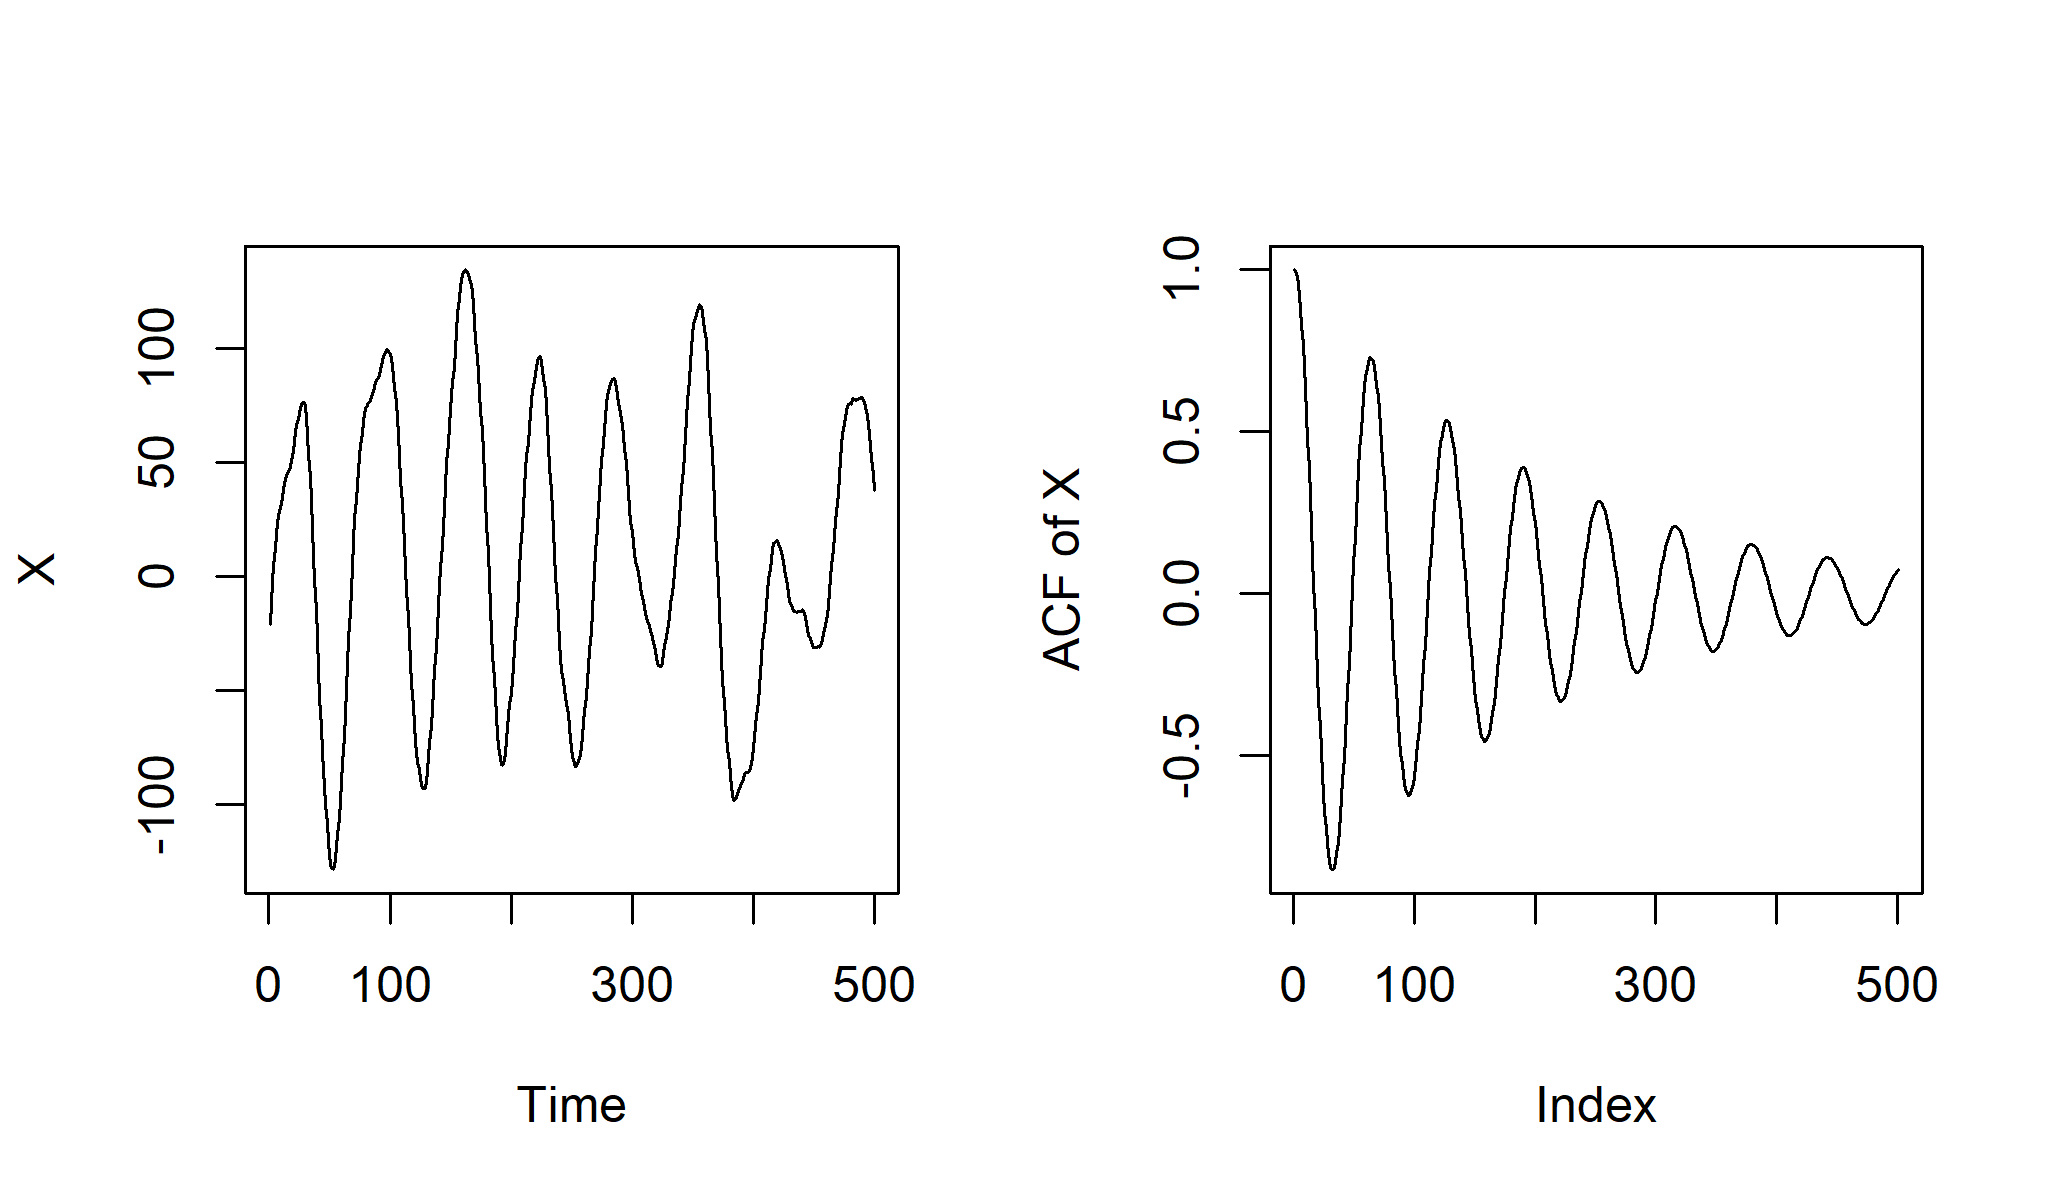
\includegraphics{figure/intro-quasi_periodic-1} \end{center}
\todo[inline]{Approx half-life of 150 b/c it starts at 1 and decays to about 0.5 at 150 in ACF plot}
\begin{itemize}
\item
  Quasi-periodic fluctuations are said to be ``phase locked'' as long as
  the random peturbations are not able to knock the oscillations away
  from being close to their initial phase.
\item
  Eventually, the randomness should mean that the process is equally
  likely to have any phase, regardless of the initial phase.
\end{itemize}

\begin{center}\rule{0.5\linewidth}{\linethickness}\end{center}

\begin{center}\rule{0.5\linewidth}{\linethickness}\end{center}

\subsubsection{Question: What is the timescale on which the simulated
model shows phase locked
behavior?}\label{question-what-is-the-timescale-on-which-the-simulated-model-shows-phase-locked-behavior}

\begin{itemize}
\tightlist
\item
  Equivalently, on what timescale does the phase of the fluctuations
  lose memory of its initial phase?
\end{itemize}

\begin{center}\rule{0.5\linewidth}{\linethickness}\end{center}

\begin{center}\rule{0.5\linewidth}{\linethickness}\end{center}


\end{document}
